\documentclass[11pt]{article}

\usepackage{a4wide}
\usepackage[utf8]{inputenc}
\usepackage[russian]{babel}
\usepackage{graphicx}
\usepackage{amsmath}
\usepackage{amsthm}
\usepackage{amssymb}

\newtheorem{theorem}{Теорема}
\newtheorem{definition}{Определение}
\newtheorem{proposition}{Утверждение}

\newcommand*{\hm}[1]{#1\nobreak\discretionary{}{\hbox{$\mathsurround=0pt #1$}}{}}
\newcommand\abs[1]{\left\lvert#1\right\rvert}
\newcommand{\scalar}[2]{\left<#1,#2\right>}
\newcommand{\norm}[1]{\left\lVert #1 \right\lVert}
\newcommand{\const}{\ensuremath{\operatorname{const}}}
\newcommand{\sgn}{\ensuremath{\operatorname{sgn}}}
\renewcommand{\d}[1]{\ensuremath{\operatorname{d}\!{#1}}}

\begin{document}
\thispagestyle{empty}

\begin{center}
\ \vspace{-3cm} \newline
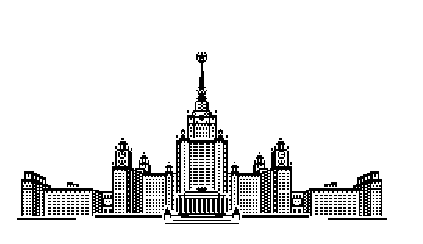
\includegraphics[width=0.5\textwidth]{msu.eps}\\
{\scshape Московский государственный университет имени М.~В.~Ломоносова}\\
Факультет вычислительной математики и кибернетики\\
Кафедра системного анализа

\vfill

{\LARGE Отчёт по практикуму <<Оптимальное управление>>} \newline
%\vspace{1cm}
{\Huge\bfseries Задание 3: построение множества достижимости}
\end{center}

\vspace{1cm}
\begin{flushright}
\large
\textit{Студент 315 группы}\\
В.~С.~Терёшин\\
%\vspace{5mm}
%\textit{Руководитель практикума}\\
%к.ф.-м.н., доцент П.~П.~Петров
\end{flushright}

\vfill
\begin{center}
Москва, 2014
\end{center}
\pagebreak
\tableofcontents
\pagebreak
\section{Постановка задачи}
Задано обыкновенное дифференциальное уравнение:
$$
\ddot{x} + x + \sin \dot{x} + x \sin x^3 = u,
$$
где $x \in \mathbb{R}$, $u \in \mathbb{R}$. На возможные значения параметра $u$ наложено ограничение: $u \in [-\alpha; \alpha]$. Задан начальный момент времени $t_0 = 0$ и начальная позиция $x(t_0) = \dot{x}(t_0) \hm= 0$. Необходимо построить множество достижимости $X(t, t_0, x(t_0), \dot{x}(t_0))$ (множество пар $(x(t), \dot{x}(t))$ в классе программных управлений в заданный момент времени $t \geqslant t_0$).
\begin{enumerate}
\item
Необходимо написать в среде \texttt{Matlab} функцию \texttt{reachset(alpha, t)}, которая по заданным параметрам $\alpha > 0$, $t \geqslant t_0$ рассчитывает приближённо множество достижимости $X(t, t_0, x(t_0), \dot{x}(t_0))$. На выходе функции --- два массива \texttt{X} и \texttt{Y} с упорядоченными координатами точек многоугольника, образующего границу искомого множества. Точки в этих массивах должны быть упорядочены так, чтобы результаты работы функции без дополнительной обработки можно было подавать на вход функциям визуализации (например, \texttt{plot}). Предусмотреть такой режим работы функции, при котором она возвращает также координаты линий переключений оптимального управления (с возможностью их визуализации).
\item
Необходимо реализовать функцию \texttt{reachsetdyn(alpha, t1, t2, N, filename)}, которая, используя функцию \texttt{reachset(alpha, t)}, строит множества достижимости для моментов времени $\tau_i = t_1 + \tfrac{t_2 - t_1}{N}, i = 0, 1, \ldots, N$. Здесь $t_2 \geqslant t_1 \geqslant t_0$, $N$ --- натуральное число. Для каждого момента времни $\tau_i$ фукнция должна отобразить многоугольник, аппроксимирующий границу множества достижимости. Результат работы функции должен быть сохранён в виде видео-файла \texttt{filename.avi}. Необходимо также предусмотреть вариант работы функции (при отсутствии параметра \texttt{filename}) без сохранения в файл, с выводом непосредственно на экран. Как частный случай, функция должна иметь возможность строить границу множества достижимости в один фиксированный момент времени (при $t_1 = t_2$).
\end{enumerate}
\section{Теория}
\subsection{Принцип максимума Понтрягина}
Обозначая $x_1 = x$, запишем данное уравнение в виде:
$$
\left\{
\begin{aligned}
\dot{x_1} = x_2, \\
\dot{x_2} = u - x_1 - \sin x_2 - x_1 \sin x_1^3 = u - f(x_1, x_2), \\
x_1(0) = x_2(0) = 0.
\end{aligned}
\right.
$$
\begin{definition}[Множество достижимости]
Множеством достижимости $X(T, t_0, x_0)$ назувается множество всех таких точек $x \in \mathbb{R}^2$, что существует такое измеримое управление $u(t)$, что для любого $t \in [t_0; T]$ $u(t) \in \mathcal{P}$ и под его воздействием система за время $T - t_0$ переходит из точки $x_0$ в точку $x$.
\end{definition}

Существование управления $u^*$, переводящего систему из точки $x_0$ в точку $x$ за время $t$, эквивалентно существованию оптимального по быстродействию управления, переводящего систему в точку $x$ за время $t^* \leqslant t$.

Рассмотрим любое допустимое управление $\tilde{u}(t) \in \mathcal{P}$. За время $T - t_0$ под действием этого управления данная система переведёт точку $x_0$ в некоторую точку $\tilde{x}$ множества достижимости $X(T, t_0, x_0)$. Для допустимой точки $\tilde{x}$ существует оптимальное по быстродействию управление $\tilde{u}^*$, переводящее систему в точку $\tilde{x}$ за время $t^* \leqslant T - t_0$.

Если $t^* = T - t_0$, то управление $\tilde{u}(t)$ оптимально и точка $\tilde{x}$ принадлежит множеству, содержащему границу множества достижимости $\partial X(t, t_0, x_0)$, иначе $\tilde{x}$ --- внутренняя точка множества достижимости $X(t, t_0, x_0)$.

Сформулируем принцип максимума Понтрягина для задачи быстродействия на отрезке $[x_0, \tilde{x}]$, где $\tilde{x}$ --- произвольная допустимая точка. Выпишем функцию Гамильтона-Понтрягина:
$$
H(t, x, u, \psi) = \psi_1 x_2 + \psi_2(u - f(t, x, u)) = \psi_1 x_2 + \psi_2(u - x_1 - \sin x_2 - x_1 \sin x_1^3).
$$
\begin{theorem}[Принцип максимума Понтрягина]
Пусть $\left( x^*(t), u^*(t) \right)$ --- оптимальная по быстродействию пара. Тогда существует непрерывная вектор-функция $\psi(t)$ (называемая сопряжённой) такая, что выполнены:
\begin{enumerate}
\item
условие сопряжённости:
$$
\dot{\psi_i}(t) = -\frac{\partial H(t, x^*(t), u^*(t), \psi(t))}{\partial x_i}, \; \; \; i = 1, 2,
$$
условие невырожденности:
$$
\psi(t) \neq 0 \; \; \forall t.
$$
\item
условие максимума:
$$
\sup \limits_{u \in \mathcal{P}} H(t, x^*(t), u(t), \psi(t)) = H(t, x^*(t), u^*(t), \psi(t)) = M(t, x^*(t), \psi(t));
$$
\item
вдоль оптимальной траектории функция Гамильтона-Понтрягина постоянна и неотрицательна:
$$
M(t, x^*(t), \psi(t)) = M(t_0, x_0, \psi(t_0)) = \const \geqslant 0.
$$
\end{enumerate}
\end{theorem}

Запишем сопряжённую систему:
$$
\left\{
\begin{aligned}
\dot{\psi_1} = \psi_2(1 + \sin x_1^3 + 3 x_1^3 \cos x_1^3), \\
\dot{\psi_2} = \psi_2 \cos x_2 - \psi_1.
\end{aligned}
\right.
$$

Заметим, что полученная система однородна, а значит, $\psi(t)$ определяется с точностью до умножения на константу. Также домножение $\psi(t)$ на положительную константу не влияет на выполнение принципа максимума.

Из условия максимума следует, что оптимальное управление имеет вид:
$$
u^*(t) = \begin{cases}
\alpha, & \psi_2(t) > 0, \\
[-\alpha; \alpha], & \psi_2(t) = 0, \\
-\alpha, & \psi_2(t) < 0.
\end{cases}
$$
Отсутствие особых режимов тривиальным образом выводится из сопряжённой системы и невырожденности $\psi(t)$. Значит, $u^*(t) = \sgn(\psi_2(t))$.

Итак, любую достижимую точку $\tilde{x}$ можно получить, решая данную систему с оптимальным управлением $u^*(t)$ указанного вида за время $t^* \leqslant T - t_0$, причём при $t^* = T - t_0$ точка $\tilde{x}$ лежит во множестве, содержащем границу множества достижимости $X(T, t_0, x_0)$. Поэтому для получения $\partial X(t, t_0, x_0)$ построим концы всех траекторий, полученных при управлении $u^*(t)$ за время $T - t_0$.
\subsection{Исследование переключений оптимального управления}
Из формулы для оптимального управления $u^*(t)$ следует, что при $\psi_2(t) = 0$ происходит переключение. Докажем, что число переключений в рассматриваемой задаче конечно.
\begin{theorem}[О конечном числе переключений]
Пусть $\psi(t)$ --- сопряжённая функция. Тогда $\psi_2(t)$ имеет конечное число нулей на $[t_0, T]$.
\end{theorem}
\begin{proof}[Доказательство]
Предположим противное: пусть $\psi_2(t)$ имеет бесконечное число нулей на отрезке $[t_0, T]$. Тогда для последовательности $t_n$: $\psi_2(t_n) = 0$ существует предельная точка $\tilde{t} \in [t_0, T]$. По теореме Лагранжа существует $\tau_n \in [t_n, t_{n+1}]$: $\psi_2(t_{n+1}) - \psi({t_n}) = \dot{\psi_2}(\tau_n)(t_{n+1} - t_n) = 0 \Rightarrow \; \; \dot{\psi_2}(\tau_n) = 0$. В силу непрерывности функций $\psi_2$, $\dot{\psi_2}$ получим: $\psi_2(\tilde{t}) = \dot{\psi_2}(\tilde{t}) = 0 \Rightarrow \; \; \psi_1(\tilde{t}) = 0 \Rightarrow \; \; \psi(\tilde{t}) = 0$.
Что противоречит условию невырожденности $\psi$. Значит, $\psi_2(t)$ имеет конечное число нулей на $[t_0, T]$.
\end{proof}

\begin{theorem}[О смене знака управления]
Пусть $u(t)$ удовлетворяет принципу максимума на $[t_0, T]$, $(x_1(t), x_2(t))$ --- траектория системы, $(\psi_1(t), \psi_2(t))$ --- сопряжённая вектор-функция. Пусть в некоторой точке $\xi \in (t_0, T)$ $\psi_2(\xi) = 0$. Тогда если $x_2(\xi) > 0$, то $\dot{\psi_2}(\xi) < 0$, если $x_2(\xi) < 0$, то $\dot{\psi_2(\xi) > 0}$.
\end{theorem}
\begin{proof}[Доказательство]
$$
M(t, x^*(t), \psi(t))\bigr\rvert_{t = \xi} = \psi_1(\xi) x_2(\xi) + \abs{\psi_2(\xi)} - \psi_2(\xi)f(x_1, x_2) = \psi_1 x_2 \geqslant 0.
$$
В силу условия сопряжённости $\dot{\psi_2}({\xi}) = -\psi_1$. Отсюда следует утверждение теоремы.
\end{proof}

Из теоремы 3 следует, что если переключение происходит при $x_2(t) > 0$, то управление переключается с $u = \alpha$ на $u = -\alpha$, а при $x_2(t) < 0$ наоборот.

\begin{theorem}[О чередовании нулей]
Пусть $u(t)$ удовлетворяет принципу максимума на $[t_0, T]$, $(x_1(t), x_2(t))$ --- траектория данной системы, $(\psi_1(t), \psi_2(t))$ --- сопряжённая вектор-функция. Тогда для любых $t_1$, $t_2$ таких, что $t_0 \leqslant t_1 \leqslant t_2 \leqslant T$ справедливы следующие утверждения:
\begin{enumerate}
\item
$\psi_2(t_1) = \psi_2(t_2) = 0, \; \psi_2(t) \neq 0$ при $t \in [t_1, t_2], x_2(t_1) = 0 \; \; \Rightarrow \; \; x_2(t_2) = 0$;
\item
$\psi_2(t_1) = \psi_2(t_2) = 0, \; \psi_2(t) \neq 0$ при $t \in [t_1, t_2], x_2(t_1) \neq 0 \; \; \Rightarrow \; \; x_2(t_2) \neq 0$ и существует $\tau \in [t_1, t_2]: x_2(\tau) = 0$;
\item
$x_2(t_1) = x_2(t_2) = 0, \; x_2(t) \neq 0$ при $t \in [t_1, t_2], \psi_2(t_1) = 0 \; \; \Rightarrow \; \; \psi_2(t_2) = 0$;
\item
$x_2(t_1) = x_2(t_2) = 0, \; x_2(t) \neq 0$ при $t \in [t_1, t_2], \psi_2(t_1) \neq 0 \; \; \Rightarrow \; \; \psi_2(t_2) \neq 0$ и существует $\tau \in [t_1, t_2]: \psi_2(\tau) = 0$;
\end{enumerate}
\end{theorem}
\begin{proof}[Доказательство]
\begin{enumerate}
\item
По принципу максимума вдоль оптимальной траектории функция Гамильтона-Понтрягина построянна:
$$
\left.
\begin{aligned}
M(t, x^*(t), \psi(t)) = \psi_1(t_1) x_2(t_1) = \psi_1(t_2) x_2(t_2) = 0 \\
\psi_2(t_2) = 0 \Rightarrow \psi_1(t_2) \neq 0
\end{aligned}
\right|
\Rightarrow x_2(t_2) = 0.
$$
\item
$$
\left.
\begin{aligned}
M(t, x^*(t), \psi(t)) = \psi_1(t_1) x_2(t_1) = \psi_1(t_2) x_2(t_2) \\
\psi_2(t_2) = 0, \Rightarrow \psi_1(t_1) \neq 0, \psi_1(t_2) \neq 0 \\
x_2(t_2) \neq 0
\end{aligned}
\right|
\Rightarrow x_2(t_2) \neq 0.
$$

Так как $\psi_2(t_1) = \psi_2(t_2) = 0$ --- два соседних нуля непрерывной функции (следовательно, есть смена монотонности) и в силу условия сопряжённости:
$$
\psi_1(t_1) \psi_1(t_2) = \dot{\psi_2}(t_1) \dot{\psi_2}(t_2) \leqslant 0.
$$
В силу невырожденности $\psi(t)$ получим строгое неравенство: $\psi_1(t_1) \psi_1(t_2) < 0$. Следовательно, $x_2(t_1) x_2(t_2) < 0$, из чего для непрерывной функции получим, что существует $\tau \in [t_1, t_2]: x_2(\tau) = 0$.
\item
Из принципа максимума следует, что
$$
M(t, x^*(t), \psi(t)) = \psi_1(t) x_2(t) + \abs{\psi_2(t)} - \psi_2(t)f(x_1(t), x_2(t)) = x_2(t) \psi_1(t) + \dot{x_2}(t)\psi_2(t) = \const \leqslant 0.
$$
Следовательно, $x_2(t_1)\psi_1(t_1) + \dot(x_2)(t_1)\psi_2(t_1) = x_2(t_2)\psi_1(t_2) + \dot(x_2)(t_2) \psi_2(t_2)$. Учитывая, что $x_2(t_1) = x_2(t_2) = 0$, получим
$$
\dot{x_2}(t_1)\psi_2(t_1) = \dot{x_2}(t_2)\psi_2(t_2). \label{star}
$$
Так как $t_1$, $t_2$ --- соседние нули фукнции $x_2(t)$, то $\dot{x_2}(t_1) \neq 0$, $\dot{x_2}(t_2) \neq 0$. Поэтому из того, что $\psi_2(t_1) = 0$, следует $\psi_2(t_2) = 0$.
\item
Из \ref{star} следует, что $\psi_2(t_2) \neq 0$. Если предположить, что $\psi_2(t)$. не обращается в нуль нигде на $[t_1, t_2]$, то из \ref{star} получим $\dot{x_2}(t_1)\dot{x_2}(t_2) > 0$, что невозможно, так как $t_1$, $t_2$ --- соседние нули функции $x_2(t)$ (должна быть смена монотонности).
\end{enumerate}
\end{proof}

Из теоремы 4 следует, что корни функций $\psi_2(t)$ и $x(t)$ либо чередуются, либо совпадают.
\subsection{Алгоритм построения границы множества достижимости}
\begin{definition}[Линий переключения]
Линией переключения называется множество всех точек в области управляемости, в которых происходит переключение управления.
\end{definition}

Рассмотрим системы $S_+$ и $S_-$:
$$
\left\{
\begin{aligned}
\dot{x_1} = x_2, \\
\dot{x_2} = \alpha - f(x_1, x_2);
\end{aligned}
\right., \; \; \;
\left\{
\begin{aligned}
\dot{x_1} = x_2, \\
\dot{x_2} = -\alpha - f(x_1, x_2);
\end{aligned}
\right.
$$

Пусть сначала $u = \alpha$. Выпустим из начальной позиции $x_0 = 0$ траекторию $W_+^1$ решения системы $S_+$. Переключение управления происходит в момент времени $t: \; \psi_2(t) = 0$. Из теоремы о чередовании нулей следует, что $\psi_2(t)$ обнулится не позже $x_2(t)$, поэтому организуем перебор времён первого переключения $\xi_1$ по равномерной сетке $(0, \tau]$, где $\tau \in [0, T]: \; x_2(\tau) = 0$ и $x_2(t) \neq 0$ при $t \in (0, \tau)$ или, если $x_2(t) = \neq 0$ на $[0, T]$, возьмём $\tau = T$. По теореме о смене знака управления $\dot{\psi_2}(\xi_1) < 0$, так как переключение осуществляется с $u = 1$ на $u = -1$. Следовательно, $\psi_1(\xi_1) = -\dot{\psi_2}(\xi_1) > 0$, а $\psi(t)$ определяется с точностью до умножения на положительную константу, поэтому возьмём $\psi_1(\xi_1) = 1$. Получим задачу Коши для системы $S_-$ и сопряжённой системы с начальными условиями $(x_1(\xi_1), x_2(\xi_1), 1, 0)$. Так как точки траектории $W_+^1$ на отрезке времени $(0, \tau)$ рассматриваются как точки переключения, то они принадлежат линии переключения.

Далее, решая полученную задачу Коши, ищем $\xi_2: \psi_2(\xi_2) = 0$ --- второе время переключения $\psi_2(t)$. В этот момент времени происходит переключение на систему $S_+$ с начальными условиями $(x_1(\xi_2), x_2(\xi_2), -1, 0)$. Добавим точку $x(\xi_2)$ к линии переключения.

Продолжаем процесс до тех пор, пока $t < T$. По теореме о конечном числе нулей функции $\psi_2(t)$ на $[0, T]$ процесс не бесконечный.

Аналогично рассматривается случай, когда система стартует с управлением $u = -\alpha$.

Концы полученных траекторий в момент времени $T$ образуют кривую, которая содержит границу множества достижимости $X(T, t_0, x_0)$, так как построенные траектории удовлетворяют принципу максимуму, следовательно, построены заведомо все оптимальные по быстродействию траектории.
\section{Техническая реализация}

Дифференциальные уравнения в процессе нахождения множества достижимости будем решать численно с помощью функции \texttt{ode45}.

Так как полученное множество концов траекторий только содержит искомую границу множества достижимости, но не совпадает с ней, была реализована функция, которая удаляет из замкнутой ломаной самопересечения. Она действует следующим образом:
\begin{enumerate}
\item
Найдём вершину ломаной, заведомо входящей в границу множества достижимости. Например, такой точка является самый нижний из самых левых концов траектории.
\item
Будем обходить ломаную, начиная с этой вершины. Для каждого последующего отрезка проверим, пересекается ли он с каким-то из предыдущих. Если да, то удалим все звенья ломаной между этими.
\end{enumerate}
\section{Примеры работы}
\begin{enumerate}
\item
$\alpha = 0.1$, $t = 1.0, \; t = 3.0, \; t = 6.0$:

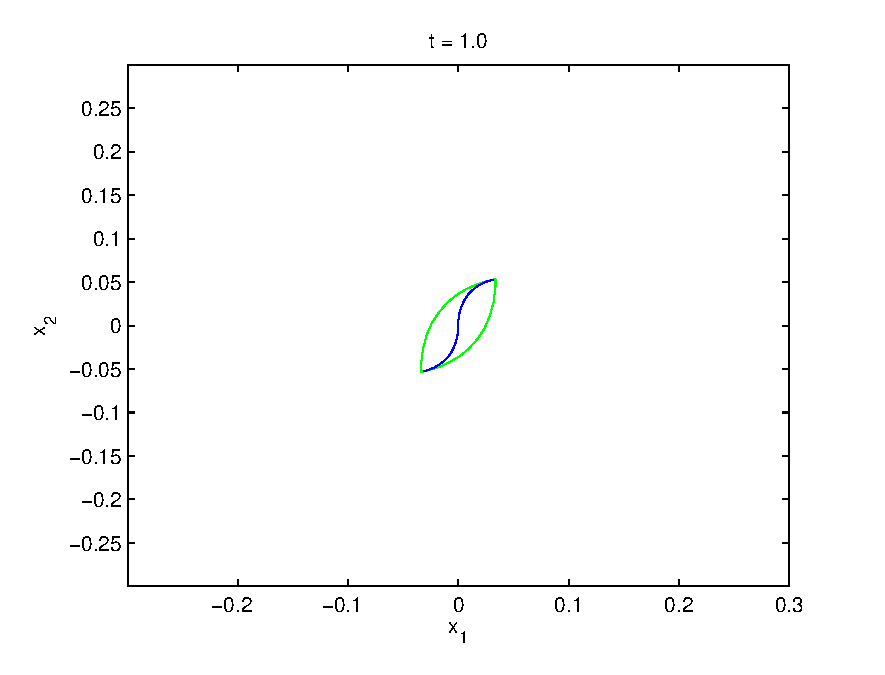
\includegraphics[scale=1.0]{pics/a0.1t1.eps}

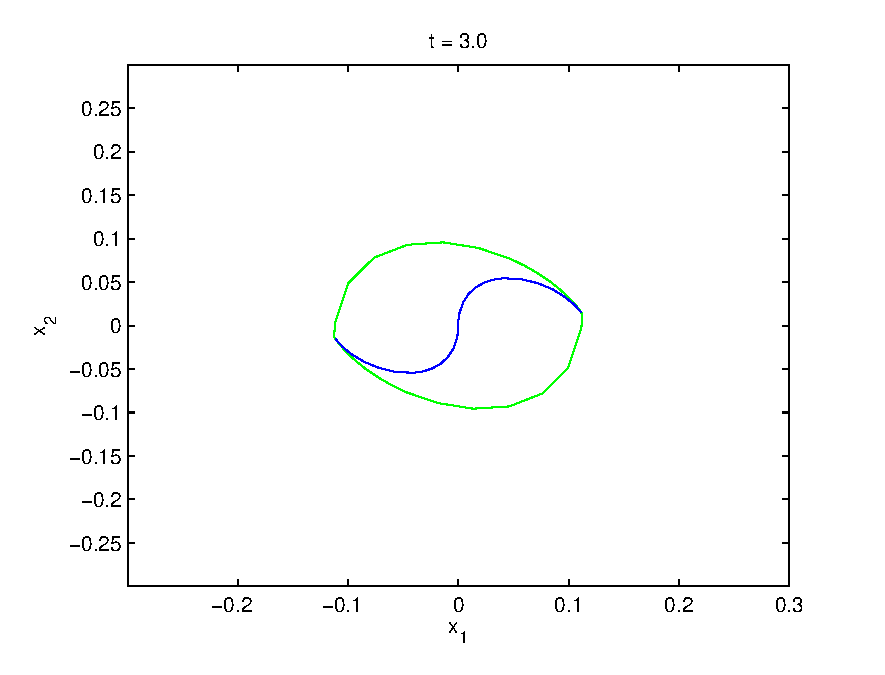
\includegraphics[scale=1.0]{pics/a0.1t3.eps}

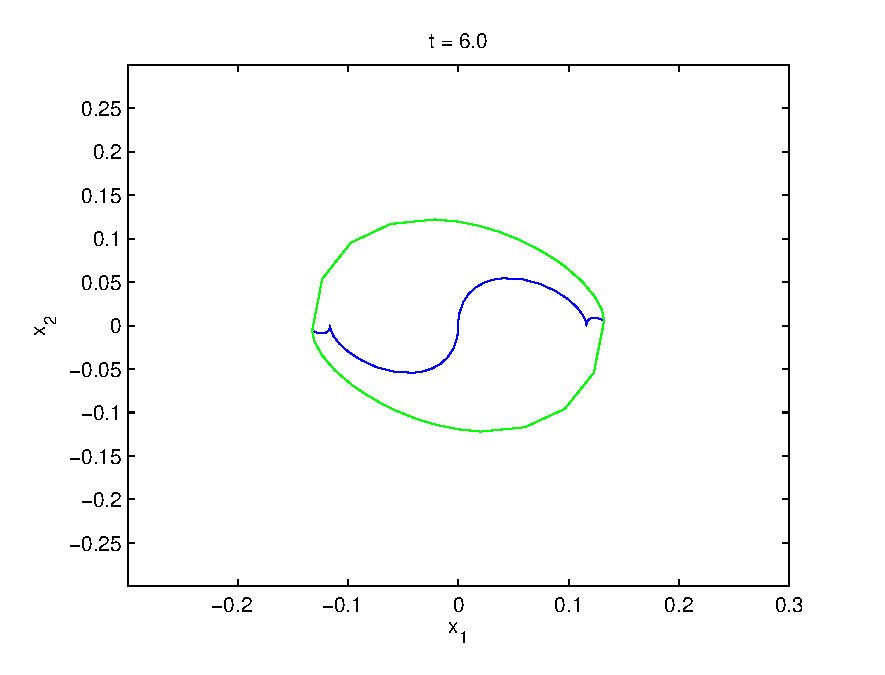
\includegraphics[scale=1.0]{pics/a0.1t6.eps}

\item
$\alpha = 1.0$, $t = 1.5, \; t = 2.5, \; t = 3.7$:

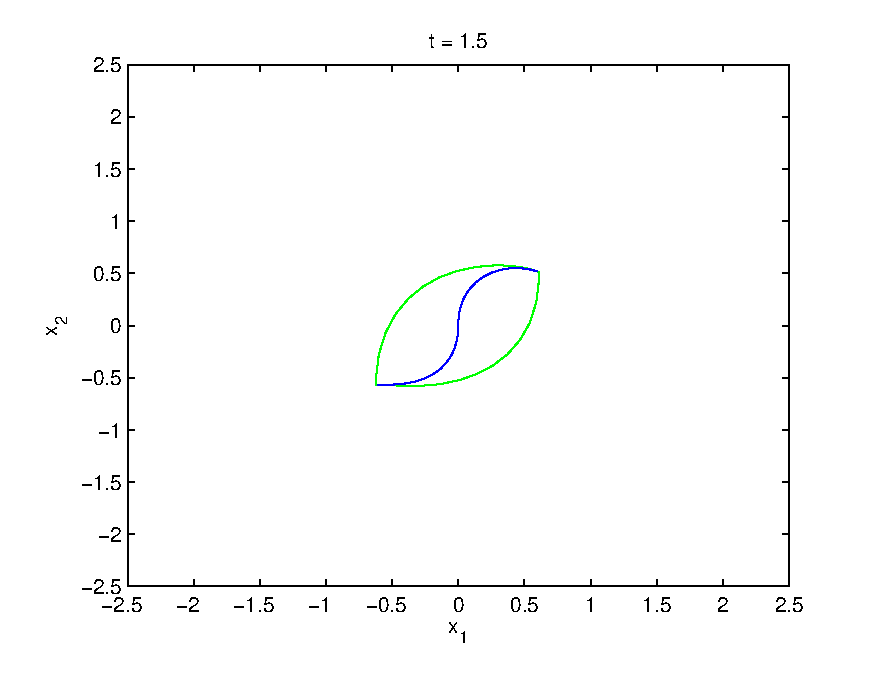
\includegraphics[scale=1.0]{pics/a1t1.5.eps}

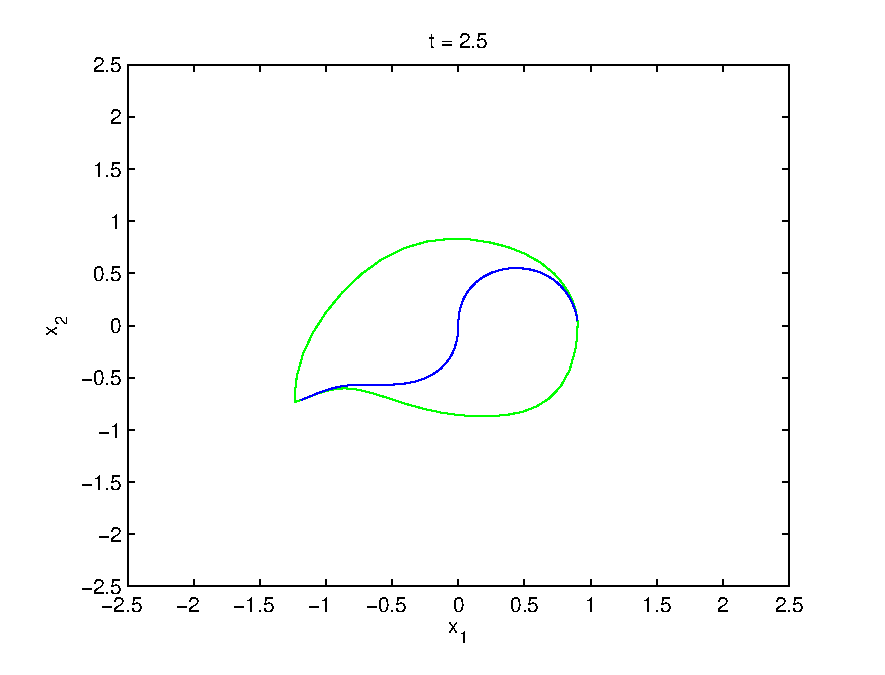
\includegraphics[scale=1.0]{pics/a1t2.5.eps}

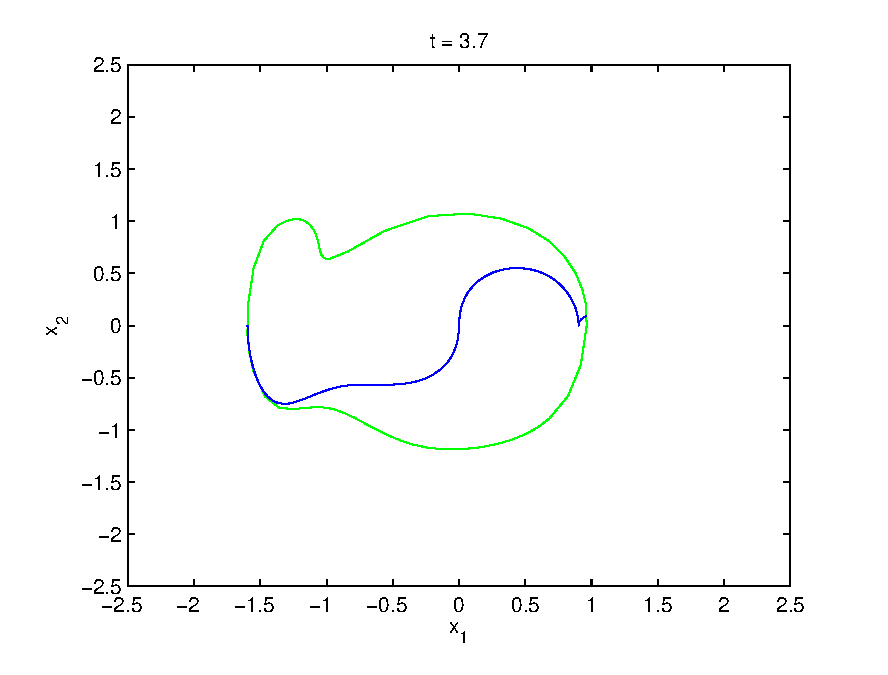
\includegraphics[scale=1.0]{pics/a1t3.7.eps}

\item
$\alpha = 2.0$, $t = 1.0, \; t = 1.5, \; t = 2.0$:

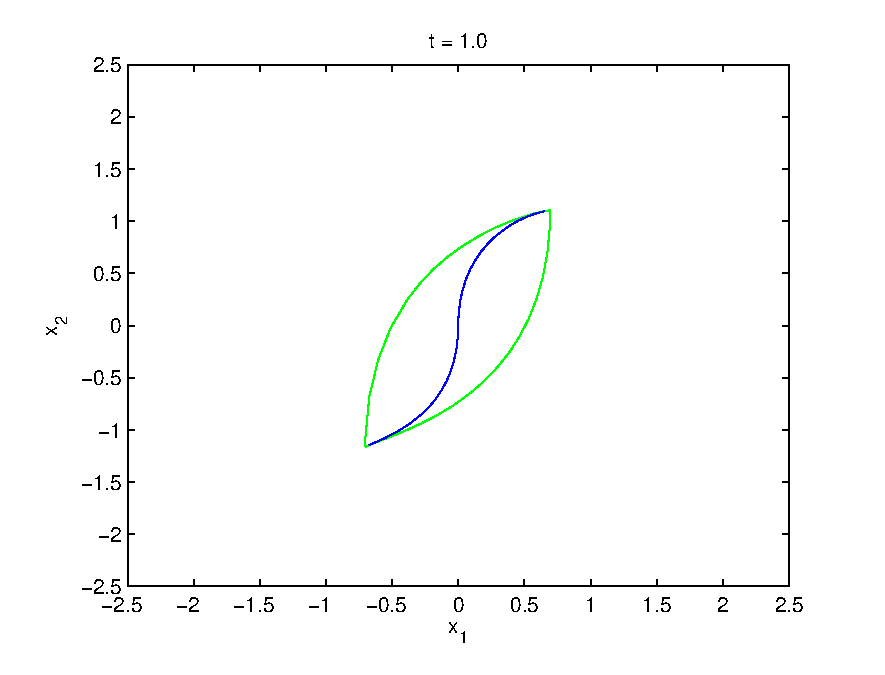
\includegraphics[scale=1.0]{pics/a2t1.eps}

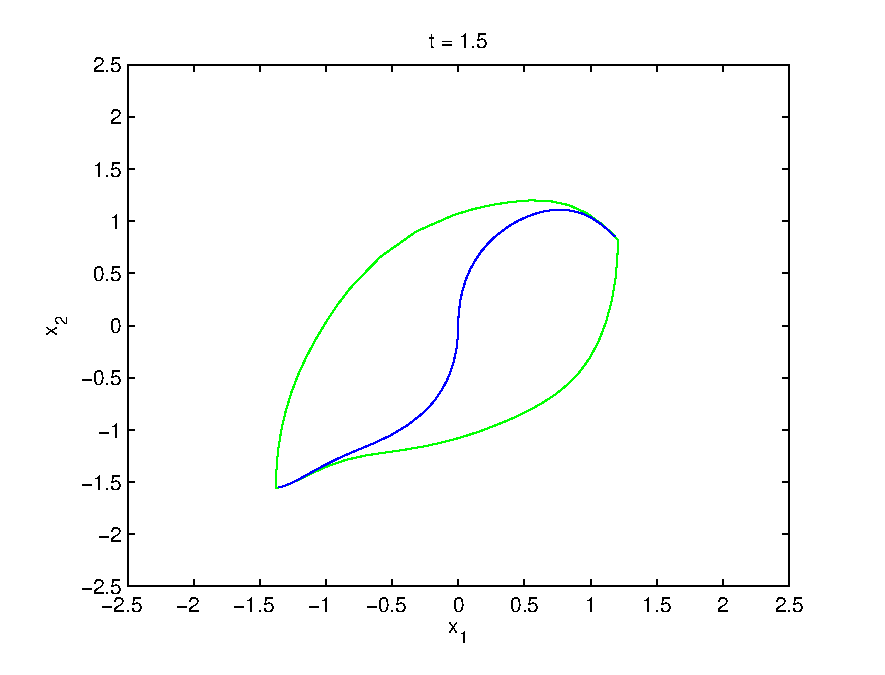
\includegraphics[scale=1.0]{pics/a2t1.5.eps}

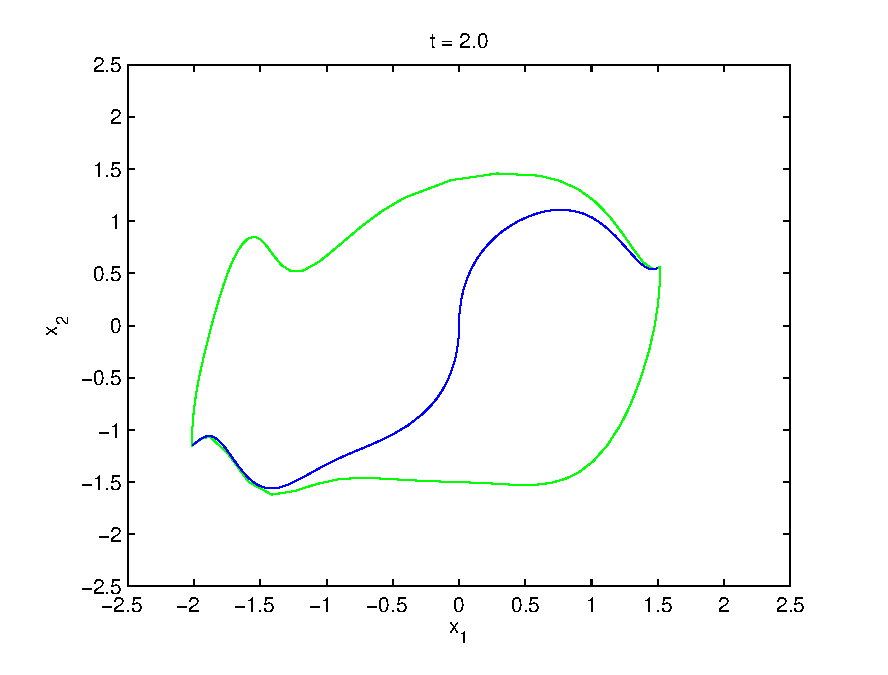
\includegraphics[scale=1.0]{pics/a2t2.eps}

\end{enumerate}
\pagebreak
\addcontentsline{toc}{section}{Список литературы}
\begin{thebibliography}{99}
	\bibitem{PBGM} Понтрягин~Л.~С., Болтянский~В.~Г., Гамкрелидзе~Р.~В., Мищенко~Е.~Ф. Математическая теория оптимальных процессов. М:~ Наука, 1976.
	\bibitem{Arutyunov} Арутюнов~А.~В., Магарил~--Ильяев~Г.~Г., Тихомиров~В.~М. Принцип максимума Понтрягина. М: Факториал Пресс, 2006.
\end{thebibliography}
\end{document}
